\documentclass[3p, authoryear, review]{elsarticle} %review=doublespace preprint=single 5p=2 column
%%% Begin My package additions %%%%%%%%%%%%%%%%%%%
\usepackage[hyphens]{url}

  \journal{Submitted to Journal} % Sets Journal name


\usepackage{lineno} % add
\providecommand{\tightlist}{%
  \setlength{\itemsep}{0pt}\setlength{\parskip}{0pt}}

\usepackage{graphicx}
%%%%%%%%%%%%%%%% end my additions to header

\usepackage[T1]{fontenc}
\usepackage{lmodern}
\usepackage{amssymb,amsmath}
\usepackage{ifxetex,ifluatex}
\usepackage{fixltx2e} % provides \textsubscript
% use upquote if available, for straight quotes in verbatim environments
\IfFileExists{upquote.sty}{\usepackage{upquote}}{}
\ifnum 0\ifxetex 1\fi\ifluatex 1\fi=0 % if pdftex
  \usepackage[utf8]{inputenc}
\else % if luatex or xelatex
  \usepackage{fontspec}
  \ifxetex
    \usepackage{xltxtra,xunicode}
  \fi
  \defaultfontfeatures{Mapping=tex-text,Scale=MatchLowercase}
  \newcommand{\euro}{€}
\fi
% use microtype if available
\IfFileExists{microtype.sty}{\usepackage{microtype}}{}
\usepackage{natbib}
\bibliographystyle{apalike}
\usepackage{longtable,booktabs,array}
\usepackage{calc} % for calculating minipage widths
% Correct order of tables after \paragraph or \subparagraph
\usepackage{etoolbox}
\makeatletter
\patchcmd\longtable{\par}{\if@noskipsec\mbox{}\fi\par}{}{}
\makeatother
% Allow footnotes in longtable head/foot
\IfFileExists{footnotehyper.sty}{\usepackage{footnotehyper}}{\usepackage{footnote}}
\makesavenoteenv{longtable}
\ifxetex
  \usepackage[setpagesize=false, % page size defined by xetex
              unicode=false, % unicode breaks when used with xetex
              xetex]{hyperref}
\else
  \usepackage[unicode=true]{hyperref}
\fi
\hypersetup{breaklinks=true,
            bookmarks=true,
            pdfauthor={},
            pdftitle={USTM Resiliency Sensitivity Analysis},
            colorlinks=false,
            urlcolor=blue,
            linkcolor=magenta,
            pdfborder={0 0 0}}
\urlstyle{same}  % don't use monospace font for urls

\setcounter{secnumdepth}{5}
% Pandoc toggle for numbering sections (defaults to be off)

% Pandoc citation processing

% Pandoc header
\usepackage{booktabs}



\begin{document}
\begin{frontmatter}

  \title{USTM Resiliency Sensitivity Analysis}
    \author[Brigham Young University]{Gregory Macfarlane\corref{1}}
   \ead{gregmacfarlane@byu.edu} 
    \author[Brigham Young University]{Natalie Gray}
   \ead{nat.gray2000@gmail.com} 
      \address[Brigham Young University]{Civil and Environmental Engineering Department, 430 Engineering Building, Provo, Utah 84602}
      \cortext[1]{Corresponding Author}
  
  \begin{abstract}
  This is where the abstract should go.
  \end{abstract}
   \begin{keyword} Sensitivity Analysis Resiliency Latin Hypercube Sampling\end{keyword}
 \end{frontmatter}

\hypertarget{questions}{%
\section{Questions}\label{questions}}

There exists uncertainty in travel demand models. This is known by transportation planners but the majority do not use any particular method to quantify it. This uncertainty exists to some extent by the variance among input parameters. A coefficient of variation can be used to approximate the standard deviation of the inputs, which then provides a range of values that are possible for model input \citep{zhao2002propagation}. A sampling method can then be used to determine the possible combinations of parameter variance. Two popular sampling methods are Monte Carlo (MC) simulation and Latin Hypercube Sampling (LHS). MC simulation is capable of providing full variance probability, but requires large computations to be effective on a large scale model. LHS reduces the amount of variants needed, but the amount of reduction is unknown. \citep{yang2013sensitivity}

The research questions are therefore:

\begin{itemize}
\tightlist
\item
  Using a dummy travel demand model, can Latin Hypercube Sampling simplify the iterations needed to approximate random sampling methods (e.g., Monte Carlo simulation)?
\item
  Does this method of sampling have few enough iterations for statewide model application?
\end{itemize}

\hypertarget{methods}{%
\section{Methods}\label{methods}}

To examine the effects of parameter input sensitivity, a 25 zone dummy model was created using data from the \href{https://github.com/ActivitySim/activitysim}{ActivitySim GitHub repository}. The skims data was used to get the values between zones for the distance, the single occupancy vehicle (SOV) AM time, the walk distance, and the walk to local bus total AM time. Auto time was simplified using the SOV AM time, nonmotorized uses walking distance multiplied by a factor of average walking speed, and transit time uses the walk to local bus time. The ActivitySim household data was also used and then organized so that it was capped at 4 persons, 3 vehicles, and 2 workers per household. If the value was larger than that capacity it was marked as the high values.

ActivitySim doesn't have trip productions so \href{https://github.com/byu-transpolab/nhts2017}{2017 National Household Travel Survey data} (NHTS2017) can be used to approximate them. Only weekday trips are used and the household sizes, vehicles, and workers are capped to the same extent as the ActivitySim households. The data was summarized by household sizes, vehicles and workers, and the weighted mean of each trip purpose was taken. The three trip purposes used are Home Based Work (HBW), Home Based Other (HBO), and Non-Home Based (NHB). The NHTS2017 approximated productions are then applied to each household based on size, vehicles, and workers.

Next mode choice parameters (constants and coefficients) are generated. The base values were obtained from the USTM Resiliency model. These values are shown in Table \ref{tab:MCcoeff} and Table \ref{tab:MCconst}.

\begin{table}

\caption{\label{tab:MCcoeff}Mode Choice Coefficients}
\centering
\begin{tabular}[t]{l|r|r|r}
\hline
Name & HBW & HBO & NHB\\
\hline
CIVTT & -0.0450 & -0.0350 & -0.0400\\
\hline
CCOST & -0.0016 & -0.0016 & -0.0016\\
\hline
CWALK1 & -0.0900 & -0.0700 & -0.0800\\
\hline
AUTOCOST & 18.3000 & 18.3000 & 18.3000\\
\hline
\end{tabular}
\end{table}

\begin{table}

\caption{\label{tab:MCconst}Mode Choice Constants}
\centering
\begin{tabular}[t]{l|r|r|r}
\hline
Name & HBW & HBO & NHB\\
\hline
K\_TRN & -0.5140 & -0.9853 & -1.3020\\
\hline
K\_NMOT & 1.7602 & 0.5448 & -0.5359\\
\hline
\end{tabular}
\end{table}

A coefficient of variation was used to identify a standard deviation for each parameter. A set coefficient of variation of 0.30 was used for all six parameters \citep{zhao2002propagation}. The standard deviation was equal to 0.30 multiplied by the mean, where the mean values in this situation are the base scenario parameters.

The MC random sampling uses the R function of \texttt{rnorm}. LHS uses the \texttt{lhs} package in R. Since this package only chooses variables on a zero to one scale, the values given the use the following function to put the random sampling on the right scale needed for the given parameter. The full code for both methods can be found in a public
\href{https://github.com/natmaegray/ustm_resiliency_sensitivity}{GitHub repository}.

100 and 600 draws of random samples are taken, the distributions for the HBW parameters are shown in Figure \ref{fig:parameter100} and Figure \ref{fig:parameter600} respectively. These distributions show that LHS gives more normally distributed parameters with fewer draws than MC sampling.

\begin{figure}

{\centering 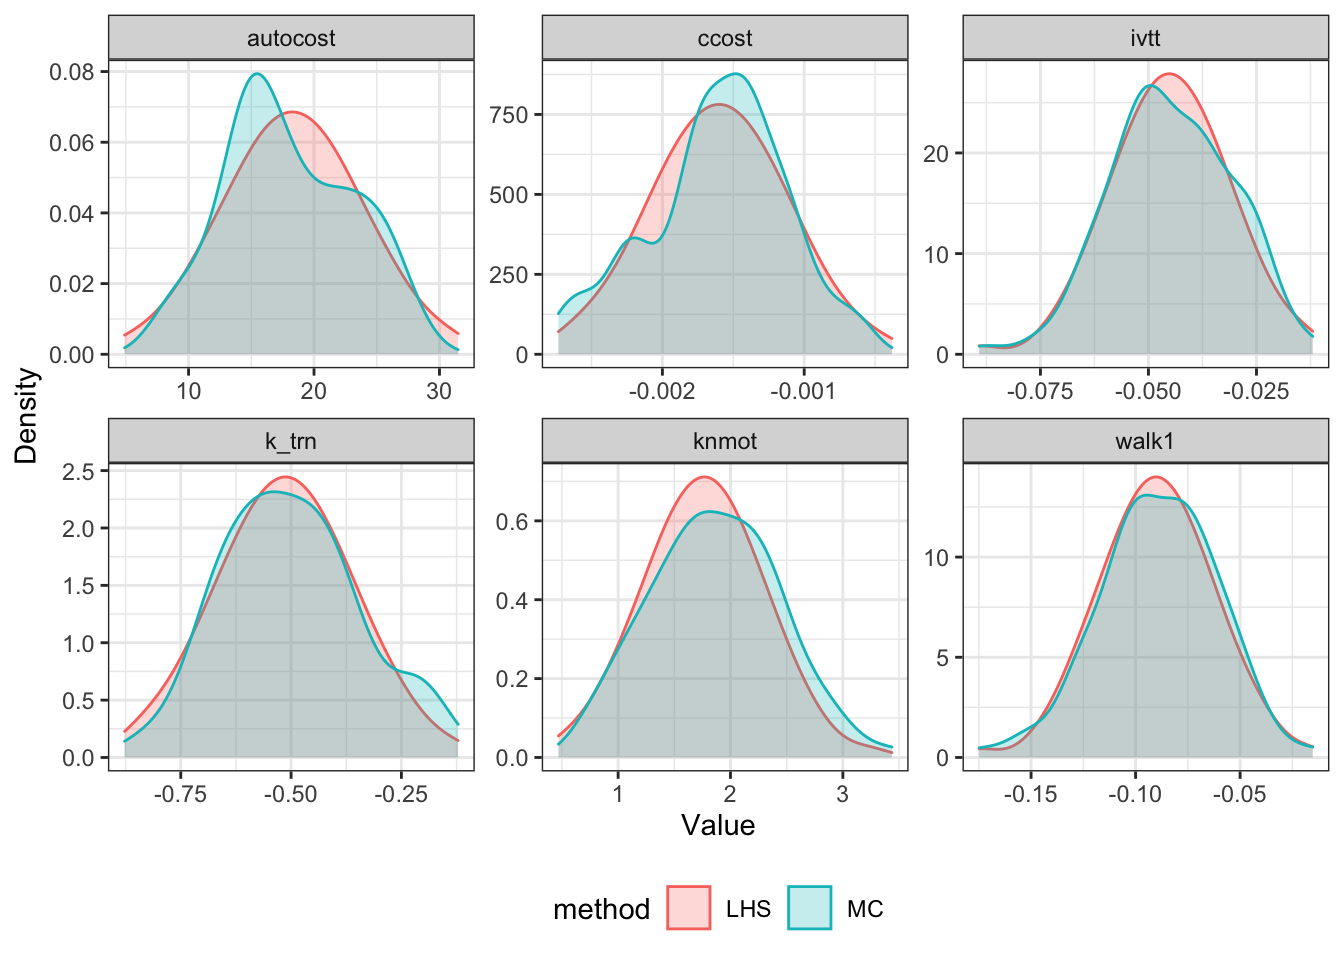
\includegraphics{ustm_resiliency_sensitivity_files/figure-latex/parameter100-1} 

}

\caption{HBW Distributions for Input Parameters with 100 Draws}\label{fig:parameter100}
\end{figure}

\begin{figure}

{\centering 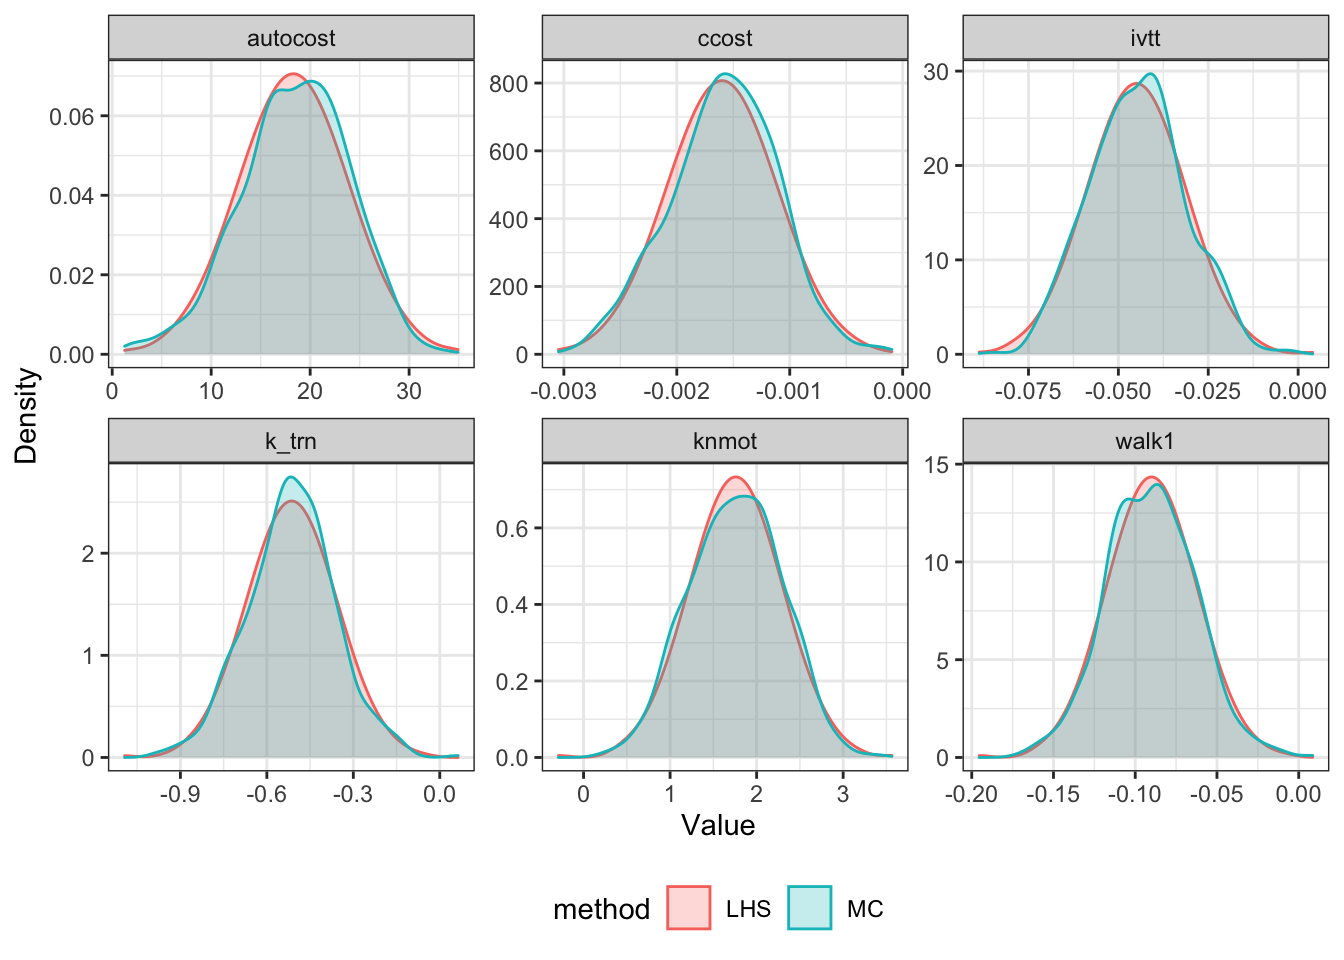
\includegraphics{ustm_resiliency_sensitivity_files/figure-latex/parameter600-1} 

}

\caption{HBW Distributions for Input Parameters with 600 Draws}\label{fig:parameter600}
\end{figure}

With these generated parameters a mode choice logsum value was calculated for each of the list types and their individual draws. The utility equations for the mode choice model are as follows:

\begin{equation}
{drive_utility} = ({coeff_ivtt}*{auto})+({coeff_cost}*{auto_cost}*{DIST})
\label{eq:driveutil}
\end{equation}
\begin{equation}
{nonmo_utility} = ({k_nmot}+ 20 * ({coeff_walk1}*{nonmotor}))
\label{eq:nonmoutil}
\end{equation}
\begin{equation}
{trans_utility} = {k_trn} + ({coeff_ivtt}*{transit})
\label{eq:transutil}
\end{equation}

These utilities were exponentiated, added together, and the natural log was taken to get a logsum value for every origin and destination pair. For each list of MC and LHS parameters the average logsum value was calculated, and the corresponding cumulative standard deviation was determined. The results of using 100 and 600 draws for each sampling method and purpose are described in the next section.

\hypertarget{findings}{%
\section{Findings}\label{findings}}

100 draws

\begin{figure}

{\centering 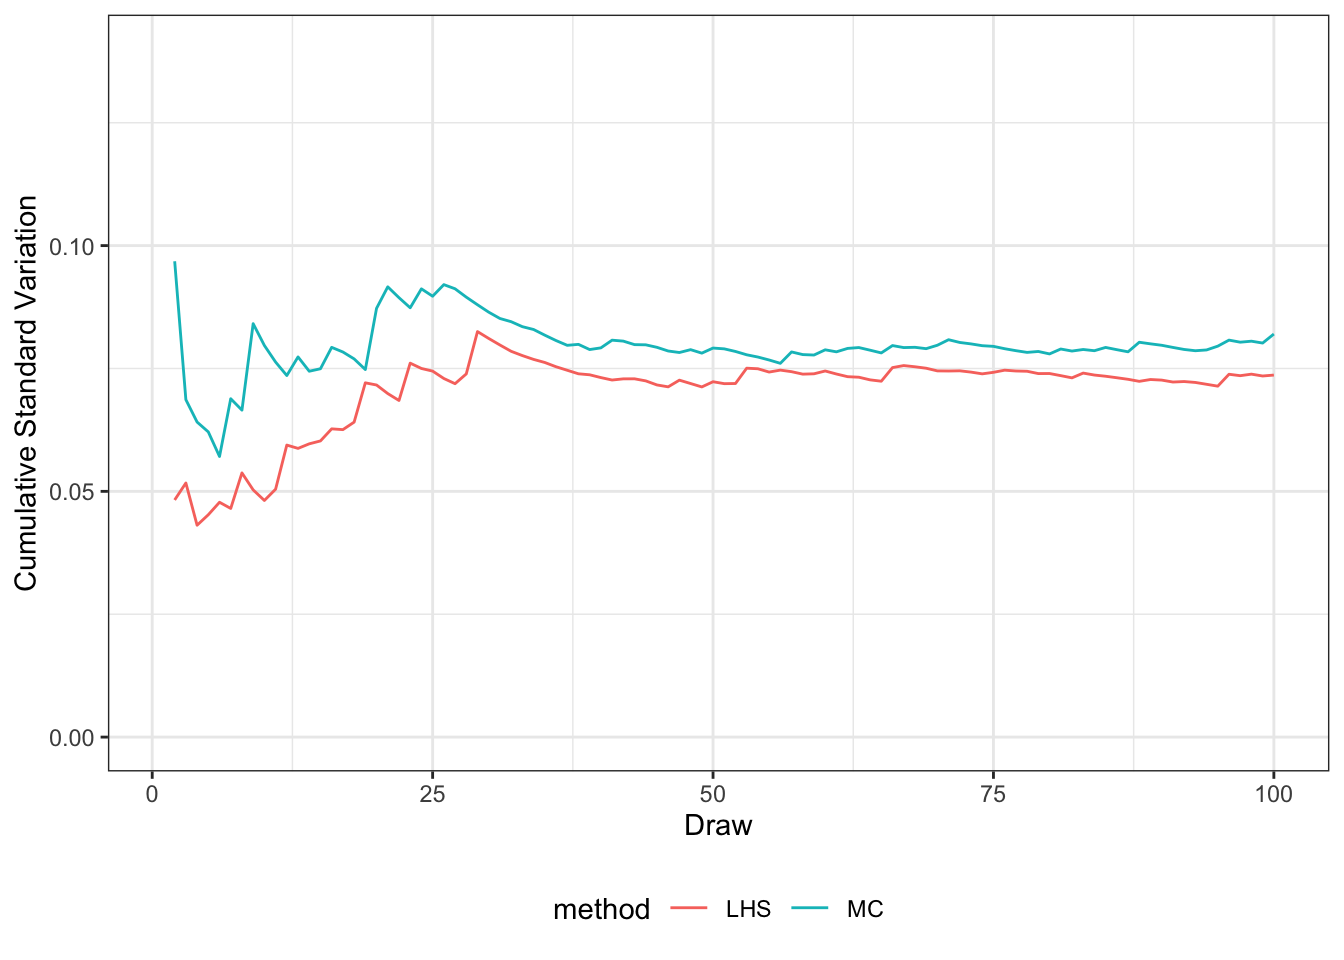
\includegraphics{ustm_resiliency_sensitivity_files/figure-latex/stats100-1} 

}

\caption{HBW Mean Logsum Standard Variation with 100 Draws}\label{fig:stats100}
\end{figure}

600 draws

\begin{figure}

{\centering 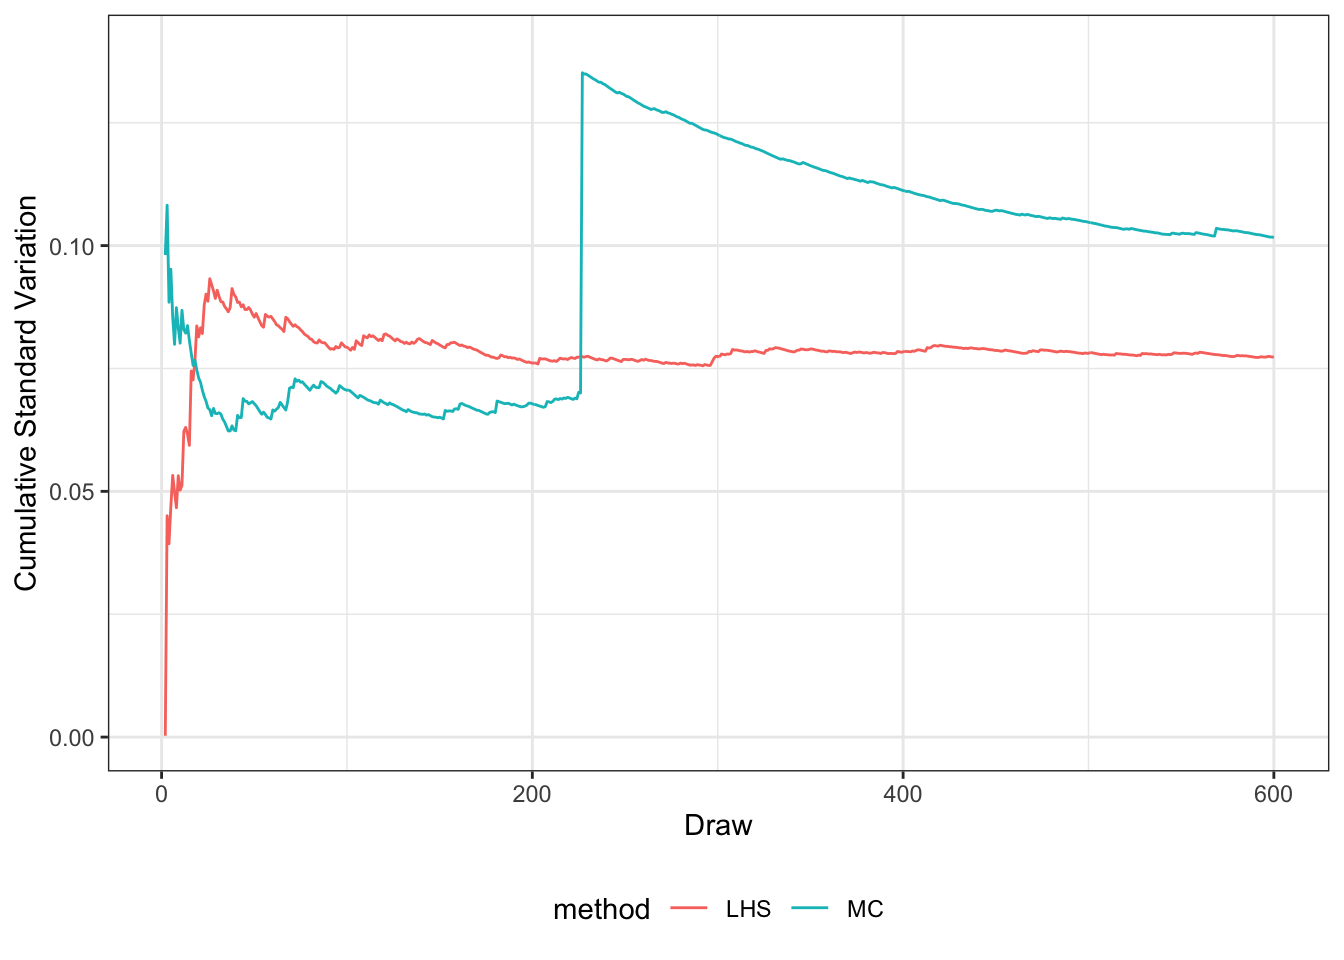
\includegraphics{ustm_resiliency_sensitivity_files/figure-latex/stats600-1} 

}

\caption{HBW Mean Logsum Standard Variation with 600 Draws}\label{fig:stats600}
\end{figure}

\begin{figure}

{\centering 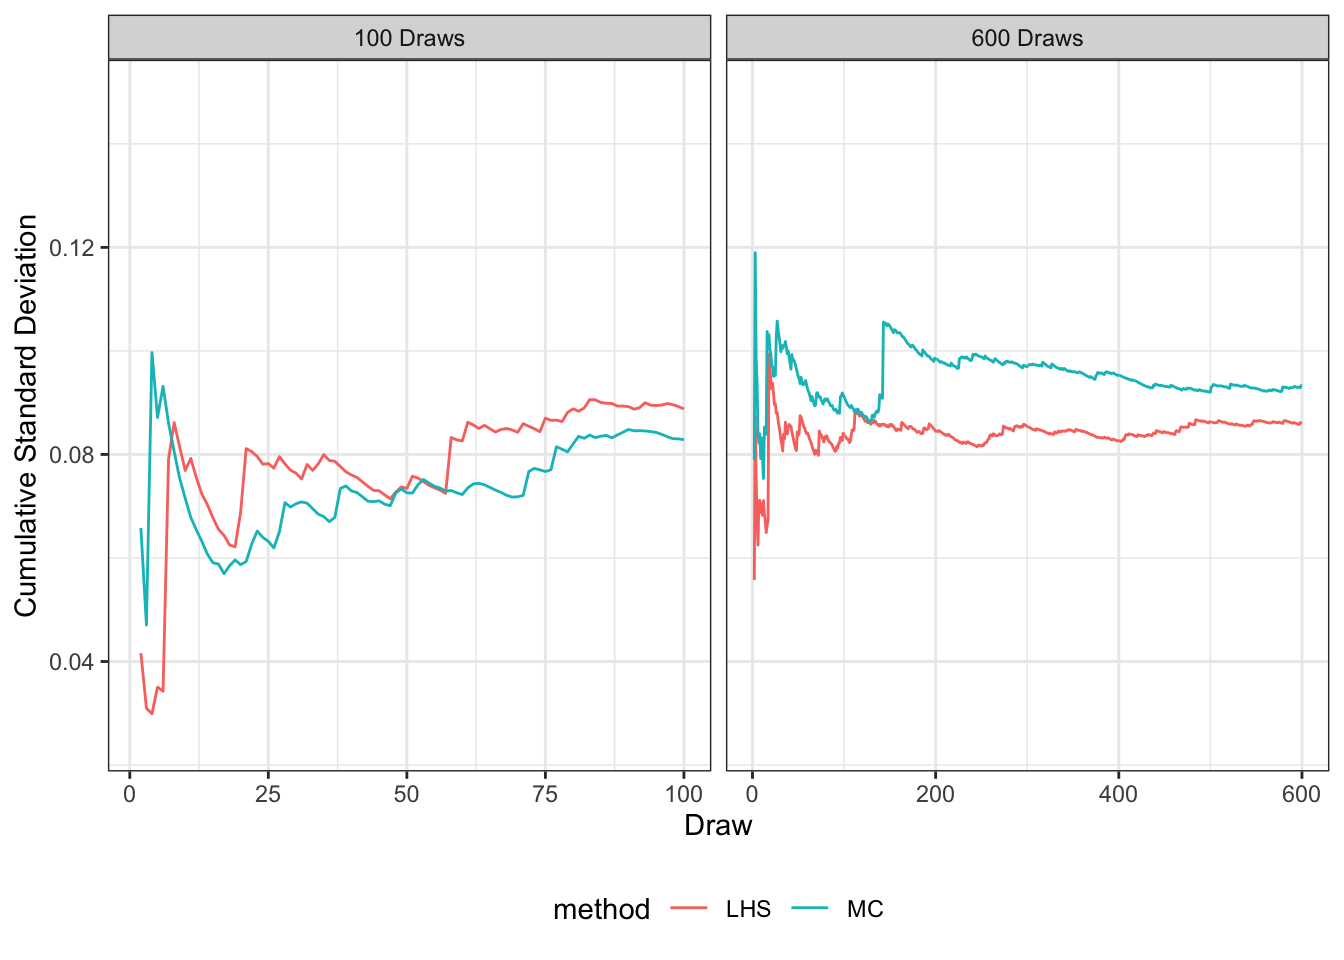
\includegraphics{ustm_resiliency_sensitivity_files/figure-latex/hbostats-1} 

}

\caption{HBO Mean Logsum Standard Variation with 100 and 600 Draws}\label{fig:hbostats}
\end{figure}

\begin{figure}

{\centering 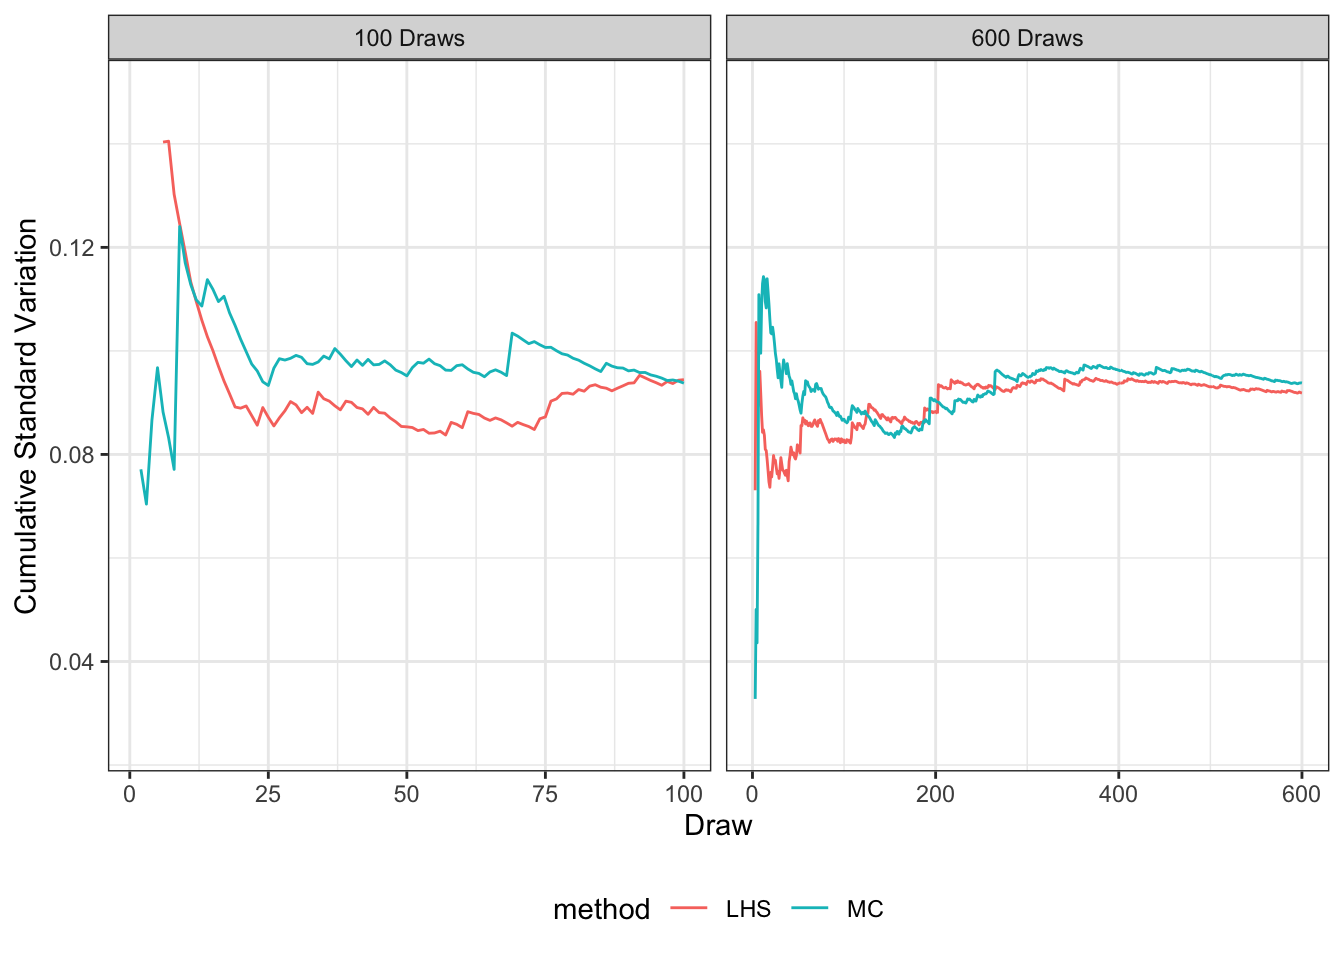
\includegraphics{ustm_resiliency_sensitivity_files/figure-latex/nhbstats-1} 

}

\caption{NHB Mean Logsum Standard Variation with 100 and 600 Draws}\label{fig:nhbstats}
\end{figure}

\bibliography{book.bib}


\end{document}
